% Options for packages loaded elsewhere
\PassOptionsToPackage{unicode}{hyperref}
\PassOptionsToPackage{hyphens}{url}
%
\documentclass[
]{book}
\usepackage{amsmath,amssymb}
\usepackage{iftex}
\ifPDFTeX
  \usepackage[T1]{fontenc}
  \usepackage[utf8]{inputenc}
  \usepackage{textcomp} % provide euro and other symbols
\else % if luatex or xetex
  \usepackage{unicode-math} % this also loads fontspec
  \defaultfontfeatures{Scale=MatchLowercase}
  \defaultfontfeatures[\rmfamily]{Ligatures=TeX,Scale=1}
\fi
\usepackage{lmodern}
\ifPDFTeX\else
  % xetex/luatex font selection
\fi
% Use upquote if available, for straight quotes in verbatim environments
\IfFileExists{upquote.sty}{\usepackage{upquote}}{}
\IfFileExists{microtype.sty}{% use microtype if available
  \usepackage[]{microtype}
  \UseMicrotypeSet[protrusion]{basicmath} % disable protrusion for tt fonts
}{}
\makeatletter
\@ifundefined{KOMAClassName}{% if non-KOMA class
  \IfFileExists{parskip.sty}{%
    \usepackage{parskip}
  }{% else
    \setlength{\parindent}{0pt}
    \setlength{\parskip}{6pt plus 2pt minus 1pt}}
}{% if KOMA class
  \KOMAoptions{parskip=half}}
\makeatother
\usepackage{xcolor}
\usepackage{color}
\usepackage{fancyvrb}
\newcommand{\VerbBar}{|}
\newcommand{\VERB}{\Verb[commandchars=\\\{\}]}
\DefineVerbatimEnvironment{Highlighting}{Verbatim}{commandchars=\\\{\}}
% Add ',fontsize=\small' for more characters per line
\usepackage{framed}
\definecolor{shadecolor}{RGB}{248,248,248}
\newenvironment{Shaded}{\begin{snugshade}}{\end{snugshade}}
\newcommand{\AlertTok}[1]{\textcolor[rgb]{0.94,0.16,0.16}{#1}}
\newcommand{\AnnotationTok}[1]{\textcolor[rgb]{0.56,0.35,0.01}{\textbf{\textit{#1}}}}
\newcommand{\AttributeTok}[1]{\textcolor[rgb]{0.13,0.29,0.53}{#1}}
\newcommand{\BaseNTok}[1]{\textcolor[rgb]{0.00,0.00,0.81}{#1}}
\newcommand{\BuiltInTok}[1]{#1}
\newcommand{\CharTok}[1]{\textcolor[rgb]{0.31,0.60,0.02}{#1}}
\newcommand{\CommentTok}[1]{\textcolor[rgb]{0.56,0.35,0.01}{\textit{#1}}}
\newcommand{\CommentVarTok}[1]{\textcolor[rgb]{0.56,0.35,0.01}{\textbf{\textit{#1}}}}
\newcommand{\ConstantTok}[1]{\textcolor[rgb]{0.56,0.35,0.01}{#1}}
\newcommand{\ControlFlowTok}[1]{\textcolor[rgb]{0.13,0.29,0.53}{\textbf{#1}}}
\newcommand{\DataTypeTok}[1]{\textcolor[rgb]{0.13,0.29,0.53}{#1}}
\newcommand{\DecValTok}[1]{\textcolor[rgb]{0.00,0.00,0.81}{#1}}
\newcommand{\DocumentationTok}[1]{\textcolor[rgb]{0.56,0.35,0.01}{\textbf{\textit{#1}}}}
\newcommand{\ErrorTok}[1]{\textcolor[rgb]{0.64,0.00,0.00}{\textbf{#1}}}
\newcommand{\ExtensionTok}[1]{#1}
\newcommand{\FloatTok}[1]{\textcolor[rgb]{0.00,0.00,0.81}{#1}}
\newcommand{\FunctionTok}[1]{\textcolor[rgb]{0.13,0.29,0.53}{\textbf{#1}}}
\newcommand{\ImportTok}[1]{#1}
\newcommand{\InformationTok}[1]{\textcolor[rgb]{0.56,0.35,0.01}{\textbf{\textit{#1}}}}
\newcommand{\KeywordTok}[1]{\textcolor[rgb]{0.13,0.29,0.53}{\textbf{#1}}}
\newcommand{\NormalTok}[1]{#1}
\newcommand{\OperatorTok}[1]{\textcolor[rgb]{0.81,0.36,0.00}{\textbf{#1}}}
\newcommand{\OtherTok}[1]{\textcolor[rgb]{0.56,0.35,0.01}{#1}}
\newcommand{\PreprocessorTok}[1]{\textcolor[rgb]{0.56,0.35,0.01}{\textit{#1}}}
\newcommand{\RegionMarkerTok}[1]{#1}
\newcommand{\SpecialCharTok}[1]{\textcolor[rgb]{0.81,0.36,0.00}{\textbf{#1}}}
\newcommand{\SpecialStringTok}[1]{\textcolor[rgb]{0.31,0.60,0.02}{#1}}
\newcommand{\StringTok}[1]{\textcolor[rgb]{0.31,0.60,0.02}{#1}}
\newcommand{\VariableTok}[1]{\textcolor[rgb]{0.00,0.00,0.00}{#1}}
\newcommand{\VerbatimStringTok}[1]{\textcolor[rgb]{0.31,0.60,0.02}{#1}}
\newcommand{\WarningTok}[1]{\textcolor[rgb]{0.56,0.35,0.01}{\textbf{\textit{#1}}}}
\usepackage{longtable,booktabs,array}
\usepackage{calc} % for calculating minipage widths
% Correct order of tables after \paragraph or \subparagraph
\usepackage{etoolbox}
\makeatletter
\patchcmd\longtable{\par}{\if@noskipsec\mbox{}\fi\par}{}{}
\makeatother
% Allow footnotes in longtable head/foot
\IfFileExists{footnotehyper.sty}{\usepackage{footnotehyper}}{\usepackage{footnote}}
\makesavenoteenv{longtable}
\usepackage{graphicx}
\makeatletter
\def\maxwidth{\ifdim\Gin@nat@width>\linewidth\linewidth\else\Gin@nat@width\fi}
\def\maxheight{\ifdim\Gin@nat@height>\textheight\textheight\else\Gin@nat@height\fi}
\makeatother
% Scale images if necessary, so that they will not overflow the page
% margins by default, and it is still possible to overwrite the defaults
% using explicit options in \includegraphics[width, height, ...]{}
\setkeys{Gin}{width=\maxwidth,height=\maxheight,keepaspectratio}
% Set default figure placement to htbp
\makeatletter
\def\fps@figure{htbp}
\makeatother
\setlength{\emergencystretch}{3em} % prevent overfull lines
\providecommand{\tightlist}{%
  \setlength{\itemsep}{0pt}\setlength{\parskip}{0pt}}
\setcounter{secnumdepth}{5}
\usepackage{booktabs}
\ifLuaTeX
  \usepackage{selnolig}  % disable illegal ligatures
\fi
\usepackage[]{natbib}
\bibliographystyle{plainnat}
\IfFileExists{bookmark.sty}{\usepackage{bookmark}}{\usepackage{hyperref}}
\IfFileExists{xurl.sty}{\usepackage{xurl}}{} % add URL line breaks if available
\urlstyle{same}
\hypersetup{
  pdftitle={Viabilidad Poblacional},
  hidelinks,
  pdfcreator={LaTeX via pandoc}}

\title{Viabilidad Poblacional}
\author{}
\date{\vspace{-2.5em}2023-07-10}

\usepackage{amsthm}
\newtheorem{theorem}{Theorem}[chapter]
\newtheorem{lemma}{Lemma}[chapter]
\newtheorem{corollary}{Corollary}[chapter]
\newtheorem{proposition}{Proposition}[chapter]
\newtheorem{conjecture}{Conjecture}[chapter]
\theoremstyle{definition}
\newtheorem{definition}{Definition}[chapter]
\theoremstyle{definition}
\newtheorem{example}{Example}[chapter]
\theoremstyle{definition}
\newtheorem{exercise}{Exercise}[chapter]
\theoremstyle{definition}
\newtheorem{hypothesis}{Hypothesis}[chapter]
\theoremstyle{remark}
\newtheorem*{remark}{Remark}
\newtheorem*{solution}{Solution}
\begin{document}
\maketitle

{
\setcounter{tocdepth}{1}
\tableofcontents
}
\hypertarget{sec-vii-andean-orchid-conference-cusco-peruxfa-24-26-noviembre-2023}{%
\chapter{VII Andean Orchid Conference, Cusco, Perú, 24-26 Noviembre 2023}\label{sec-vii-andean-orchid-conference-cusco-peruxfa-24-26-noviembre-2023}}

Lugar: Universidad Nacional de San Antonio Abad del Cusco, Perú Fecha
del taller: 24-26 Noviembre 2023

\hypertarget{impartido-por}{%
\section{\texorpdfstring{\emph{Impartido por}:}{Impartido por:}}\label{impartido-por}}

\emph{Dr.~Raymond L. Tremblay:}

Universidad de Puerto Rico Presidente de Analítica Fundación, Inc

e-mail:

\begin{itemize}
\item
  \href{mailto:raymond.tremblay@upr.edu}{\nolinkurl{raymond.tremblay@upr.edu}}
\item
  \href{mailto:tremblayanaliticafun@gmail.com}{\nolinkurl{tremblayanaliticafun@gmail.com}}
\end{itemize}

\emph{Dra. Nhora Helena Ospina-Calderón}:

Pontificia Universidad Javeriana Seccional Cali Profesora-investigadora

e-mail:

\begin{itemize}
\tightlist
\item
  \href{mailto:nhospina@javerianacali.edu.co}{\nolinkurl{nhospina@javerianacali.edu.co}}
\end{itemize}

\hypertarget{duraciuxf3n-del-taller}{%
\section{Duración del taller:}\label{duraciuxf3n-del-taller}}

Tres días con 26 horas totales de Taller-teórico practico con una
experiencia de recolección de datos en el campo (8 horas) y dos días de
taller--teórico practico y análisis datos (14 horas). Instrucción en
español.

\hypertarget{certificaciuxf3n-a-nombre-de-la}{%
\section{Certificación A nombre de la}\label{certificaciuxf3n-a-nombre-de-la}}

\begin{itemize}
\item
  Universidad Nacional San Antonio Abad del Cusco (UNSAAC)
\item
  ANALITICA Fundación Inc.~(Puerto Rico)
\end{itemize}

\hypertarget{costo-del-taller-estudiantes}{%
\section{Costo del taller Estudiantes:}\label{costo-del-taller-estudiantes}}

S/. xxx.00 nuevos soles (\$ 100.00 dol.) locales.

Profesionales: S/. xxx.00 nuevos soles (\$200.00 dol.) Estudiantes
internacional y profesionales

\hypertarget{cupo-25-personas}{%
\section{Cupo: 25 personas}\label{cupo-25-personas}}

\hypertarget{introducciuxf3n}{%
\section{Introducción}\label{introducciuxf3n}}

Este taller teórico-práctico se ofrece a los estudiantes interesados en
orquídeas y a las personas interesadas en la conservación de plantas.
Los métodos se enfocarán en el uso de las matrices de Lefkovitch para
construir modelos de historia de vida que sirven a su vez para evaluar
si una población de una especie es estable, está creciendo o se está
reduciendo. Para evaluar el crecimiento de las poblaciones se utiliza el
método de marcar y recapturar (monitorear) individuos en el campo, dicho
método se aplicará para hacer Matrices de Proyección de Poblaciones
(MPP). Se dará énfasis en el manejo para el almacenamiento y
sistematización de datos. Los datos recolectados en el campo serán
utilizados para construir una base de datos que almacene las evidencias
recogidas en el campo y funcione como insumo para calcular las matrices
de transiciones. Posterior a la construcción de matrices de transición
se analizará las tasas de crecimiento (crecimiento poblacional
intrínseco), estimando los errores y los intervalos de confianza con
distribución beta para cada una de las transiciones. También se llevará
a cabo análisis de elasticidad y la proyección del tamaño de la
población. Todos los análisis serán preparados y llevados a cabo en R,
Rstudio y RMarkdown (todos programas de distribución libre).

\hypertarget{objetivo-general}{%
\section{Objetivo general:}\label{objetivo-general}}

Introducir las bases teóricas y prácticas para la recolección de datos
de campo que permiten determinar la probabilidad de extinción de una
población.

\hypertarget{objetivos-especuxedficos}{%
\section{Objetivos específicos:}\label{objetivos-especuxedficos}}

• Conocer las bases teóricas y los métodos modernos de recolección de
datos en el campo para determinar la probabilidad de extinción de una
población.

\hfill\break
• Conocer los datos básicos y su correcta manipulación para determinar
la viabilidad de una población.

• Manipular correctamente los archivos electrónicos de datos de campo
para proponer la estructura de la población y su posterior depuración
para análisis sobre diferentes formatos.

• Aprender nociones básicas de Excel, R y RStudio para editar y analizar
conjuntos de datos para el uso con análisis de MPP.

• Construir un gráfico de ciclo de vida para la especie estudiada.

• Construir modelos demográficos que permitan predecir la dinámica
poblacional en el tiempo y generar insumos importantes para el manejo y
la conservación

• Estimar los intervalos de confianza de los parámetros del ciclo de
vida de la población.

• Utilizar la información y análisis demográfico para el diagnóstico y
predicciones de la viabilidad de las poblaciones.

• Modelar el tamaño poblacional de la población de estudio para
determinar su posible riesgo de extinción

\begin{verbatim}
\end{verbatim}

\hypertarget{introducciuxf3n-1}{%
\section{Introducción}\label{introducciuxf3n-1}}

\textbf{23 noviembre- Llegada a Cusco}

\begin{itemize}
\item
  8:00 pm- 9:15pm

  \begin{itemize}
  \tightlist
  \item
    Introducción al taller y Presentación de conceptos básicos
    (Capítulo 2; Tremblay)
  \item
    Diagrama del ciclo de vida (Capítulo 3; Ospina)
  \end{itemize}
\end{itemize}

\textbf{24 noviembre: Viaje de campo}

\begin{itemize}
\item
  Salida 6:00 am - Llegada 8:15 am.

  \begin{itemize}
  \tightlist
  \item
    Llegada al sitio de muestreo campo
  \end{itemize}
\item
  8:30am- 5:00pm.

  \begin{itemize}
  \item
    - Determinación de la especie a estudiar (Ospina y Tremblay)
  \item
    - Métodos de recolección de datos - Recolección de datos
    (Capítulo 4 y 22; Ospina y Tremblay)
  \end{itemize}
\end{itemize}

\textbf{25 noviembre:}

8:30 pm-10:30 pm

\begin{itemize}
\tightlist
\item
  - Teoria:

  \begin{itemize}
  \tightlist
  \item
    Proponer un ciclo de vida (Capítulo 3)
  \item
    Quien se reproduce y como calcular la fecundidad (Capitulo 6)
  \item
    Como se ama la matriz (3 x 3) y ejercicio (Capítulo 5)

    \begin{itemize}
    \tightlist
    \item
      Subir la matriz a mano

      \begin{itemize}
      \tightlist
      \item
        Multiplicación del vector (N en el tiempo t) con la
        matriz = Nt+1
      \end{itemize}
    \end{itemize}
  \end{itemize}
\end{itemize}

10:30am -- 12:00pm

\begin{itemize}
\tightlist
\item
  - Introducción a la teoria de MPP

  \begin{itemize}
  \tightlist
  \item
    crecimiento asimtotico (Capítulo 9)
  \item
    elasticidad (Capitulo 10)
  \item
    estructura estable (Capitulo Nuevo)
  \item
    valor reproductivo (Capitulo Nuevo)
  \end{itemize}
\end{itemize}

Almuerzo 12:00- 1:00pm

1:00pm - 2:30 pm

\begin{itemize}
\tightlist
\item
  - Organización de los datos en Excel/Numbers/Sheet, estructura de
  la población (Capítulo 4 y 22; Ospina y Tremblay)
\end{itemize}

2:30pm -- 5:30pm

\begin{itemize}
\item
  Introducción a R, RStudio y RMarkdown y paquetes de análisis.
  (Tremblay)
\item
  Subir los datos a RStudio, análisis preliminar de los datos usando
  \textbf{popdemo} y \textbf{raretrans} (Ospina y Tremblay)

  \begin{itemize}
  \tightlist
  \item
    Métodos para calcular contruir la matriz (Capítulo 8, Tremblay)
  \item
    Incluir la fecundidad (Capítulo 6)
  \item
    Matriz bayesiana a priori (Capítulo 8, Tremblay)
  \item
    Calcular los indices de \textbf{Oquidea cuscanensis}

    \begin{itemize}
    \tightlist
    \item
      crecimiento asintótico (Capítulo 9)
    \item
      elasticidad (Capítulo 10)
    \item
      estructura estable (Capítulo Nuevo)
    \item
      valor reproductivo (Capítulo Nuevo)
    \end{itemize}
  \end{itemize}
\end{itemize}

\textbf{26 noviembre:}

8:30 pm-10:30 pm

\begin{itemize}
\tightlist
\item
  - Descripción histórica del uso y aplicaciones de MPP (Capítulo 2,
  16: Tremblay)
\end{itemize}

10:30am -- 12:00pm

\begin{itemize}
\item
  Dinamica transitoria/ *transfer function* (Capítulo 12; Ospina)
\item
  Dinámica, análisis de viabilidad poblacional: el futuro de la
  especie (Capítulo 9: Tremblay)
\end{itemize}

Almuerzo 12:00- 1:00pm

1:00pm -- 4:30pm

\begin{itemize}
\tightlist
\item
  Estudio de casos

  \begin{itemize}
  \tightlist
  \item
    \emph{Caladenia xxx. Terrestre con latencia}
  \item
    \emph{Dracula chimaera}. Epífita y Terrestre
  \item
    \emph{Dendrophylax lindenii}. Epífita áfila
  \item
  \end{itemize}
\end{itemize}

4:30pm -- 5:30pm

\begin{itemize}
\tightlist
\item
  Presentaciones de trabajo
\end{itemize}

\hypertarget{materiales-necesarios}{%
\section{Materiales necesarios:}\label{materiales-necesarios}}

\begin{enumerate}
\def\labelenumi{\arabic{enumi}.}
\tightlist
\item
  Computadora portátil (Mac o PC) con Excel, R y Rstudio
\end{enumerate}

\begin{itemize}
\tightlist
\item
  Los participantes pueden trabajar en parejas en caso de que sea
  difícil conseguir una computadora portatil.\\
\item
  Es necesario acudir a las sesiones teóricas con los programas y
  paquetes previamente instalados, se enviará instrucciones y brindará
  oportuna asesoría.
\end{itemize}

\hypertarget{bibliografuxeda}{%
\section{Bibliografía}\label{bibliografuxeda}}

Gascoigne Samuel J. L., Simon Rolph, Daisy Sankey, Nagalakshmi
Nidadavolu, Adrian S. Stell Pičman, Christina M. Hernández, Matthew
Philpott, Aiyla Salam, Connor Bernard, Erola Fenollosa, Jessie McLean,
Shathuki Hetti Achchige Perera, Oliver G. Spacey, Maja Kajin, Anna C.
Vinton, C. Ruth Archer, Jean H. Burns, Danielle L. Buss, Hal Caswell,
Judy P. Che-Castaldo, Dylan Z. Childs, Pol Capdevila, Aldo Compagnoni,
Elizabeth Crone, Thomas H. G. Ezard, Dave Hodgson, Owen Jones, Eelke
Jongejans Jenni McDonald, Brigitte Tenhumberg, Chelsea C. Thomas, Andrew
J. Tyre, Satu Ramula, Iain Stott, Raymond L. Tremblay, Phil Wilson,
James W. Vaupel, and Roberto Salguero-Gómez.. 2023. \textbf{A standard
protocol to report discrete stage-structured demographic information.}
Submitted to Methods in Ecology and Evolution. In press.

Stott, I., Hodgson, D. J., \& Townley, S. (2012). \textbf{Beyond sensitivity:
nonlinear perturbation analysis of transient dynamics. Methods in
Ecology and Evolution}. 3(4), 673-684. doi:
10.1111/j.2041-210X.2012.00199.x

Stott, I., Hodgson, D. J., \& Townley, S. (2012b). \textbf{Popdemo: An R
package for population demography using projection matrix analysis.
Methods in Ecology and Evolution}, 3(5), 797-802.
\url{https://doi.org/10.1111/j.2041-210X.2012.00222.x}

Stott, I., Townley, S., \& Hodgson, D. J. (2011). \textbf{A framework for
studying transient dynamics of population projection matrix models}.
Ecology Letters, 14(9), 959-970. doi: 10.1111/j.1461-0248.2011.01659.x

Tremblay, R. L., \& Hutchings, M. J. (2002). \textbf{Population dynamics in
orchid conservation: a review of analytical methods based on the rare
species Lepanthes eltoroensis}. Orchid conservation. Kota Kinabalu:
Natural History Publications (Borneo), 183-204.

Tremblay, R. L., Raventos, J., \& Ackerman, J. D. (2015). \textbf{When
stable-stage equilibrium is unlikely: integrating transient population
dynamics improves asymptotic methods}. Annals of Botany, 116(3),
381-390. \url{doi:10.1093/aob/mcv031}

Tremblay, R. L., Tyre, A. J., Pérez, M. E., \& Ackerman, J. D. (2021).
\textbf{Population projections from holey matrices: Using prior information to
estimate rare transition events}. Ecological Modelling, 447, 109526.
\url{https://doi.org/10.1016/j.ecolmodel.2021.109526}.

\textbf{Que conocemos de estas especies?}

Especies reportadas de trabajo

\begin{itemize}
\item
  Cyrtochilum cimiciferum (Rchb.f.) Dalström (Tiene una gran poblacion
  )
\item
  Cyrtochilum myanthum (Lindl.) Kraenzl.1917
\item
  \emph{Epidendrum chalmersii} Hágsater \& Ric. Fernández 2013 (endémico de
  la región Cusco)
\item
  \emph{Epidendrum syringothyrsus} Rchb.f. ex Hook.f. 1875
\item
  \emph{Pleurothallis casapensis} Lindl. 1842
\item
  \emph{Habenaria} sp.
\item
  \emph{Cyclopogon} sp.
\end{itemize}

\hypertarget{hello-bookdown}{%
\chapter{Hello bookdown}\label{hello-bookdown}}

All chapters start with a first-level heading followed by your chapter title, like the line above. There should be only one first-level heading (\texttt{\#}) per .Rmd file.

\hypertarget{a-section}{%
\section{A section}\label{a-section}}

All chapter sections start with a second-level (\texttt{\#\#}) or higher heading followed by your section title, like the sections above and below here. You can have as many as you want within a chapter.

\hypertarget{an-unnumbered-section}{%
\subsection*{An unnumbered section}\label{an-unnumbered-section}}
\addcontentsline{toc}{subsection}{An unnumbered section}

Chapters and sections are numbered by default. To un-number a heading, add a \texttt{\{.unnumbered\}} or the shorter \texttt{\{-\}} at the end of the heading, like in this section.

\hypertarget{cross}{%
\chapter{Cross-references}\label{cross}}

Cross-references make it easier for your readers to find and link to elements in your book.

\hypertarget{chapters-and-sub-chapters}{%
\section{Chapters and sub-chapters}\label{chapters-and-sub-chapters}}

There are two steps to cross-reference any heading:

\begin{enumerate}
\def\labelenumi{\arabic{enumi}.}
\tightlist
\item
  Label the heading: \texttt{\#\ Hello\ world\ \{\#nice-label\}}.

  \begin{itemize}
  \tightlist
  \item
    Leave the label off if you like the automated heading generated based on your heading title: for example, \texttt{\#\ Hello\ world} = \texttt{\#\ Hello\ world\ \{\#hello-world\}}.
  \item
    To label an un-numbered heading, use: \texttt{\#\ Hello\ world\ \{-\#nice-label\}} or \texttt{\{\#\ Hello\ world\ .unnumbered\}}.
  \end{itemize}
\item
  Next, reference the labeled heading anywhere in the text using \texttt{\textbackslash{}@ref(nice-label)}; for example, please see Chapter \ref{cross}.

  \begin{itemize}
  \tightlist
  \item
    If you prefer text as the link instead of a numbered reference use: \protect\hyperlink{cross}{any text you want can go here}.
  \end{itemize}
\end{enumerate}

\hypertarget{captioned-figures-and-tables}{%
\section{Captioned figures and tables}\label{captioned-figures-and-tables}}

Figures and tables \emph{with captions} can also be cross-referenced from elsewhere in your book using \texttt{\textbackslash{}@ref(fig:chunk-label)} and \texttt{\textbackslash{}@ref(tab:chunk-label)}, respectively.

See Figure \ref{fig:nice-fig}.

\begin{Shaded}
\begin{Highlighting}[]
\FunctionTok{par}\NormalTok{(}\AttributeTok{mar =} \FunctionTok{c}\NormalTok{(}\DecValTok{4}\NormalTok{, }\DecValTok{4}\NormalTok{, .}\DecValTok{1}\NormalTok{, .}\DecValTok{1}\NormalTok{))}
\FunctionTok{plot}\NormalTok{(pressure, }\AttributeTok{type =} \StringTok{\textquotesingle{}b\textquotesingle{}}\NormalTok{, }\AttributeTok{pch =} \DecValTok{19}\NormalTok{)}
\end{Highlighting}
\end{Shaded}

\begin{figure}

{\centering 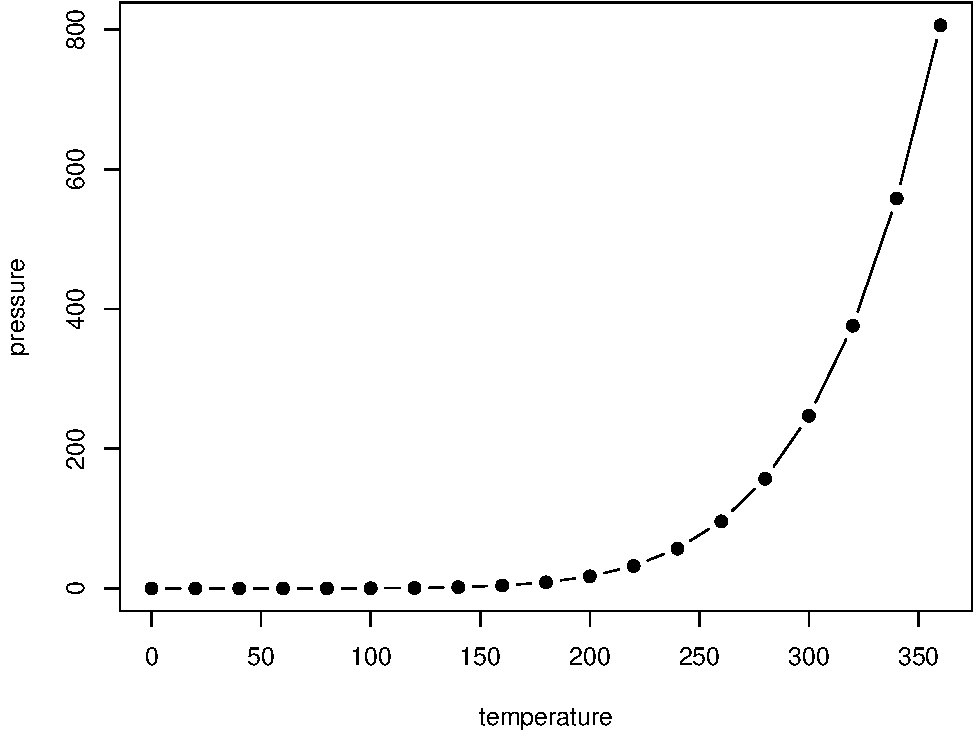
\includegraphics[width=0.8\linewidth]{_main_files/figure-latex/nice-fig-1} 

}

\caption{Here is a nice figure!}\label{fig:nice-fig}
\end{figure}

Don't miss Table \ref{tab:nice-tab}.

\begin{Shaded}
\begin{Highlighting}[]
\NormalTok{knitr}\SpecialCharTok{::}\FunctionTok{kable}\NormalTok{(}
  \FunctionTok{head}\NormalTok{(pressure, }\DecValTok{10}\NormalTok{), }\AttributeTok{caption =} \StringTok{\textquotesingle{}Here is a nice table!\textquotesingle{}}\NormalTok{,}
  \AttributeTok{booktabs =} \ConstantTok{TRUE}
\NormalTok{)}
\end{Highlighting}
\end{Shaded}

\begin{table}

\caption{\label{tab:nice-tab}Here is a nice table!}
\centering
\begin{tabular}[t]{rr}
\toprule
temperature & pressure\\
\midrule
0 & 0.0002\\
20 & 0.0012\\
40 & 0.0060\\
60 & 0.0300\\
80 & 0.0900\\
\addlinespace
100 & 0.2700\\
120 & 0.7500\\
140 & 1.8500\\
160 & 4.2000\\
180 & 8.8000\\
\bottomrule
\end{tabular}
\end{table}

\hypertarget{parts}{%
\chapter{Parts}\label{parts}}

You can add parts to organize one or more book chapters together. Parts can be inserted at the top of an .Rmd file, before the first-level chapter heading in that same file.

Add a numbered part: \texttt{\#\ (PART)\ Act\ one\ \{-\}} (followed by \texttt{\#\ A\ chapter})

Add an unnumbered part: \texttt{\#\ (PART\textbackslash{}*)\ Act\ one\ \{-\}} (followed by \texttt{\#\ A\ chapter})

Add an appendix as a special kind of un-numbered part: \texttt{\#\ (APPENDIX)\ Other\ stuff\ \{-\}} (followed by \texttt{\#\ A\ chapter}). Chapters in an appendix are prepended with letters instead of numbers.

\hypertarget{footnotes-and-citations}{%
\chapter{Footnotes and citations}\label{footnotes-and-citations}}

\hypertarget{footnotes}{%
\section{Footnotes}\label{footnotes}}

Footnotes are put inside the square brackets after a caret \texttt{\^{}{[}{]}}. Like this one \footnote{This is a footnote.}.

\hypertarget{citations}{%
\section{Citations}\label{citations}}

Reference items in your bibliography file(s) using \texttt{@key}.

For example, we are using the \textbf{bookdown} package \citep{R-bookdown} (check out the last code chunk in index.Rmd to see how this citation key was added) in this sample book, which was built on top of R Markdown and \textbf{knitr} \citep{xie2015} (this citation was added manually in an external file book.bib).
Note that the \texttt{.bib} files need to be listed in the index.Rmd with the YAML \texttt{bibliography} key.

The RStudio Visual Markdown Editor can also make it easier to insert citations: \url{https://rstudio.github.io/visual-markdown-editing/\#/citations}

\hypertarget{blocks}{%
\chapter{Blocks}\label{blocks}}

\hypertarget{equations}{%
\section{Equations}\label{equations}}

Here is an equation.

\begin{equation} 
  f\left(k\right) = \binom{n}{k} p^k\left(1-p\right)^{n-k}
  \label{eq:binom}
\end{equation}

You may refer to using \texttt{\textbackslash{}@ref(eq:binom)}, like see Equation \eqref{eq:binom}.

\hypertarget{theorems-and-proofs}{%
\section{Theorems and proofs}\label{theorems-and-proofs}}

Labeled theorems can be referenced in text using \texttt{\textbackslash{}@ref(thm:tri)}, for example, check out this smart theorem \ref{thm:tri}.

\begin{theorem}
\protect\hypertarget{thm:tri}{}\label{thm:tri}For a right triangle, if \(c\) denotes the \emph{length} of the hypotenuse
and \(a\) and \(b\) denote the lengths of the \textbf{other} two sides, we have
\[a^2 + b^2 = c^2\]
\end{theorem}

Read more here \url{https://bookdown.org/yihui/bookdown/markdown-extensions-by-bookdown.html}.

\hypertarget{callout-blocks}{%
\section{Callout blocks}\label{callout-blocks}}

The R Markdown Cookbook provides more help on how to use custom blocks to design your own callouts: \url{https://bookdown.org/yihui/rmarkdown-cookbook/custom-blocks.html}

\hypertarget{sharing-your-book}{%
\chapter{Sharing your book}\label{sharing-your-book}}

\hypertarget{publishing}{%
\section{Publishing}\label{publishing}}

HTML books can be published online, see: \url{https://bookdown.org/yihui/bookdown/publishing.html}

\hypertarget{pages}{%
\section{404 pages}\label{pages}}

By default, users will be directed to a 404 page if they try to access a webpage that cannot be found. If you'd like to customize your 404 page instead of using the default, you may add either a \texttt{\_404.Rmd} or \texttt{\_404.md} file to your project root and use code and/or Markdown syntax.

\hypertarget{metadata-for-sharing}{%
\section{Metadata for sharing}\label{metadata-for-sharing}}

Bookdown HTML books will provide HTML metadata for social sharing on platforms like Twitter, Facebook, and LinkedIn, using information you provide in the \texttt{index.Rmd} YAML. To setup, set the \texttt{url} for your book and the path to your \texttt{cover-image} file. Your book's \texttt{title} and \texttt{description} are also used.

This \texttt{gitbook} uses the same social sharing data across all chapters in your book- all links shared will look the same.

Specify your book's source repository on GitHub using the \texttt{edit} key under the configuration options in the \texttt{\_output.yml} file, which allows users to suggest an edit by linking to a chapter's source file.

Read more about the features of this output format here:

\url{https://pkgs.rstudio.com/bookdown/reference/gitbook.html}

Or use:

\begin{Shaded}
\begin{Highlighting}[]
\NormalTok{?bookdown}\SpecialCharTok{::}\NormalTok{gitbook}
\end{Highlighting}
\end{Shaded}


  \bibliography{book.bib,packages.bib}

\end{document}
